\documentclass[12pt]{report}
\usepackage[utf8]{inputenc}
\usepackage[russian]{babel}
\usepackage[14pt]{extsizes}
\usepackage{listings}
\usepackage{graphicx}
\usepackage{amsmath,amsfonts,amssymb,amsthm,mathtools} 
\usepackage{pgfplots}
\usepackage{filecontents}
\usepackage{float}
\usepackage{indentfirst}
\usepackage{eucal}
\usepackage{enumitem}
\frenchspacing

\usepackage{indentfirst} % Красная строка


\usetikzlibrary{datavisualization}
\usetikzlibrary{datavisualization.formats.functions}

\usepackage{amsmath}




% Для листинга кода:
\lstset{ %
language=C,                 % выбор языка для подсветки (здесь это С)
basicstyle=\small\sffamily, % размер и начертание шрифта для подсветки кода
numbers=left,               % где поставить нумерацию строк (слева\справа)
numberstyle=\tiny,           % размер шрифта для номеров строк
stepnumber=1,                   % размер шага между двумя номерами строк
numbersep=5pt,                % как далеко отстоят номера строк от подсвечиваемого кода
showspaces=false,            % показывать или нет пробелы специальными отступами
showstringspaces=false,      % показывать или нет пробелы в строках
showtabs=false,             % показывать или нет табуляцию в строках
frame=single,              % рисовать рамку вокруг кода
tabsize=2,                 % размер табуляции по умолчанию равен 2 пробелам
captionpos=t,              % позиция заголовка вверху [t] или внизу [b] 
breaklines=true,           % автоматически переносить строки (да\нет)
breakatwhitespace=true, % переносить строки только если есть пробел
escapeinside={\#*}{*)}   % если нужно добавить комментарии в коде
}

\usepackage[left=2cm,right=2cm, top=2cm,bottom=2cm,bindingoffset=0cm]{geometry}
% Для измененных титулов глав:
\usepackage{titlesec, blindtext, color} % подключаем нужные пакеты
\definecolor{gray75}{gray}{0.75} % определяем цвет
\newcommand{\hsp}{\hspace{20pt}} % длина линии в 20pt
% titleformat определяет стиль
\titleformat{\chapter}[hang]{\Huge\bfseries}{\thechapter\hsp\textcolor{gray75}{|}\hsp}{0pt}{\Huge\bfseries}


% plot
\usepackage{pgfplots}
\usepackage{filecontents}
\usetikzlibrary{datavisualization}
\usetikzlibrary{datavisualization.formats.functions}

\begin{document}
%\def\chaptername{} % убирает "Глава"
\thispagestyle{empty}
\begin{titlepage}
	\noindent \begin{minipage}{0.15\textwidth}
	
\includegraphics[width=\linewidth]{img/b_logo}
	\end{minipage}
	\noindent\begin{minipage}{0.9\textwidth}\centering
		\textbf{Министерство науки и высшего образования Российской Федерации}\\
		\textbf{Федеральное государственное бюджетное образовательное учреждение высшего образования}\\
		\textbf{~~~«Московский государственный технический университет имени Н.Э.~Баумана}\\
		\textbf{(национальный исследовательский университет)»}\\
		\textbf{(МГТУ им. Н.Э.~Баумана)}
	\end{minipage}
	
	\noindent\rule{18cm}{3pt}
	\newline\newline
	\noindent ФАКУЛЬТЕТ $\underline{\text{«Информатика и системы управления»}}$ \newline\newline
	\noindent КАФЕДРА $\underline{\text{«Программное обеспечение ЭВМ и информационные технологии»}}$\newline\newline\newline\newline\newline
	
	
	\begin{center}
		\noindent\begin{minipage}{1.3\textwidth}\centering
			\Large\textbf{  Отчет по лабораторной работе №4}\newline
			\textbf{по дисциплине "Операционные системы"}\newline\newline
		\end{minipage}
	\end{center}
	
	\noindent\textbf{Тема} $\underline{\text{Процессы. Системные вызовы fork() и exec()}}$\newline\newline
	\noindent\textbf{Студент} $\underline{\text{Козлова И.В.~~~~~~~~~~~~~~~~~~~~~~~~~~~~~~~~~~~~~~}}$\newline\newline
	\noindent\textbf{Группа} $\underline{\text{ИУ7-52Б~~~~~~~~~~~~~~~~~~~~~~~~~~~~~~~~~~~~~~~~~~~~~~}}$\newline\newline
	\noindent\textbf{Оценка (баллы)} $\underline{\text{~~~~~~~~~~~~~~~~~~~~~~~~~~~~~~~~~~~~~~~~~~~~~}}$\newline\newline
	\noindent\textbf{Преподаватели} $\underline{\text{Рязанова Н.Ю.~~~~~~~~~~~~~~~~~~~~~~~~~~}}$\newline\newline\newline
	
	\begin{center}
		\vfill
		Москва~---~\the\year
		~г.
	\end{center}
\end{titlepage}

\newpage
\setcounter{page}{2}
\section*{Задание №1}

Процессы-сироты. В программе создаются не менее двух потомков. В потомках вызывается sleep(). Чтобы предок гарантированно завершился раньше своих помков. Продемонстрировать с помощью соответствующего вывода информацию об идентификаторах процессов и их группе.

\begin{lstlisting}[label=some-code,caption=Процессы-сироты,language=C]
#include <stdio.h>
#include <stdlib.h>
#include <unistd.h>

#define N 2
#define TIME_SLEEP 2

#define OK 0
#define ERR_FORK -1

#define FORK_FAILURE 1

int main()
{
	int child[N];
	
	printf("Parent process start! PID: %d, GROUP: %d\n", getpid(), getpgrp());
	
	for (int i = 0; i < N; i++)
	{
		int child_pid = fork();
		
		if(child_pid == ERR_FORK)
		{
			perror("Can\'t fork()\n");
			return FORK_FAILURE;
		}
		else if (child_pid == 0)
		{
			printf("BEFORE SLEEP Child %d! PID: %d, PPID: %d, GROUP: %d \n", i + 1, getpid(), getppid(), getpgrp());
			sleep(TIME_SLEEP);
			printf("AFTER SLEEP Child %d! PID: %d, PPID: %d, GROUP: %d\n",   i + 1, getpid(), getppid(), getpgrp());
			exit(OK);
		}
		else
		{
			child[i] = child_pid;
		}
	}
	
	printf("Parent process finished! Children: %d, %d! \nParent: PID: %d, GROUP: %d\n ", child[0], child[1], getpid(), getpgrp());
	
	return OK;
}
\end{lstlisting}

\begin{figure}[H]

	\centering

	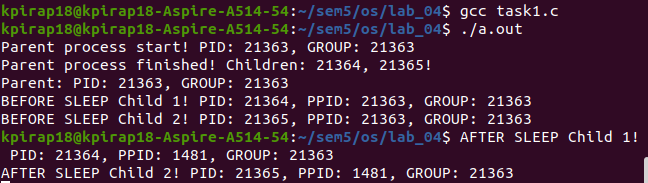
\includegraphics[width=\linewidth]{img/p1.png}
	\caption{Демонстрация работы программы (задание №1).}

	\label{fig:p1}

\end{figure}

\begin{figure}[H]
	
	\centering
	
	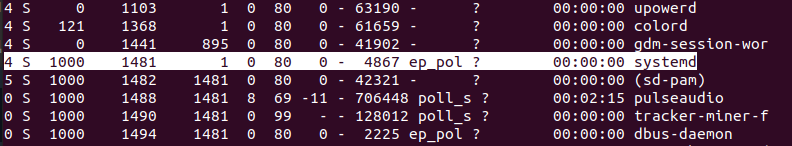
\includegraphics[width=\linewidth]{img/p1_2.png}
	\caption{Процесс, который усыновляет процессы-сироты.}
	
	\label{fig:p1_2}
	
\end{figure}


\section*{Задание №2}

Предок ждет завершения своих потомком, используя системный вызов
wait(). Вывод соответствующих сообщений на экран.

\begin{lstlisting}[label=some-code,caption=Вызов функции wait(),language=C]
#include <stdio.h>
#include <unistd.h>
#include <sys/types.h>
#include <sys/wait.h>
#include <stdlib.h>

#define N 2
#define TIME_SLEEP 2

#define OK 0
#define ERR_FORK -1

#define FORK_FAILURE 1

int main()
{
	int child[N];
	
	printf("Parent process start! PID: %d, GROUP: %d\n", getpid(), getpgrp());
	
	for (int i = 0; i < N; i++)
	{
		int child_pid = fork();
		
		if(child_pid == ERR_FORK)
		{
			perror("Can\'t fork()\n");
			return FORK_FAILURE;
		}
		else if (child_pid == 0)
		{
			printf("Child %d! PID: %d, PPID: %d, GROUP: %d\n", i + 1,   getpid(), getppid(), getpgrp());
			exit(OK);
		}     
		else
		{
			child[i] = child_pid;
		}   
	}
	
	for (int i = 0; i < N; i++)
	{
		int status;
		int statval = 0;
		
		pid_t child_pid = wait(&status);
		
		printf("Child process %d finished. Status: %d\n", child_pid, status);
		
		if (WIFEXITED(statval))
		{
			printf("Child process %d finished. Code: %d\n", i + 1, WEXITSTATUS(statval));
		}
		else if (WIFSIGNALED(statval))
		{
			printf("Child process %d finished from signal with code: %d\n", i + 1, WTERMSIG(statval));
		}
		else if (WIFSTOPPED(statval))
		{
			printf("Child process %d finished stopped. Number signal: %d\n", i + 1, WSTOPSIG(statval));
		}
	}
	
	printf("Parent process finished! Children: %d, %d! \nParent: PID: %d, GROUP: %d\n ", child[0], child[1], getpid(), getpgrp());
	
	return OK;
}
\end{lstlisting}

\begin{figure}[H]

	\centering

	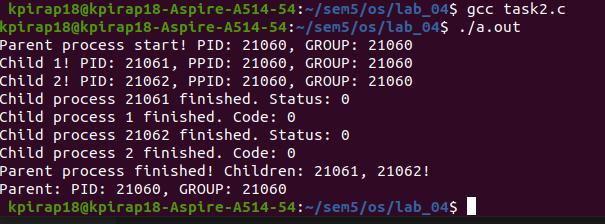
\includegraphics[width=\linewidth]{img/p2.png}
	\caption{Демонстрация работы программы (задание №2).}

	\label{fig:p2}

\end{figure}

\section*{Задание №3}

Потомки переходят на выполнение других программ. Предок ждет завершения своих потомков. Вывод соответствующих сообщений на экран.

\begin{lstlisting}[label=some-code,caption=Вызов функции execlp(),language=C]
#include <stdio.h>
#include <unistd.h>
#include <sys/types.h>
#include <sys/wait.h>
#include <stdlib.h>

#define N 2
#define TIME_SLEEP 2

#define OK 0
#define ERR_FORK -1
#define ERR_EXEC -1

#define FORK_FAILURE 1
#define EXEC_FAILURE 2

int main()
{
	int child[N];
	char *com[N] = {"./p1.exe", "./p2.exe"};
	
	printf("Parent process start! PID: %d, GROUP: %d\n", getpid(), getpgrp());
	
	for (int i = 0; i < N; i++)
	{
		int child_pid = fork();
		
		if(child_pid == ERR_FORK)
		{
			perror("Can\'t fork()\n");
			return FORK_FAILURE;
		}
		else if (child_pid == 0)
		{
			printf("Child %d! PID: %d, PPID: %d, GROUP: %d\n", i + 1, getpid(), getppid(), getpgrp());
			int rc = execlp(com[i], com[i], NULL);
			
			if (rc == ERR_EXEC)
			{
				perror("Can't exec");
				return EXEC_FAILURE;
			}
			
			exit(OK);
		}        
		else
		{
			child[i] = child_pid;
		}
	}
	
	for (int i = 0; i < N; i++)
	{
		int status;
		int statval = 0;
		
		pid_t child_pid = wait(&status);
		
		printf("Child process %d finished. Status: %d\n", child_pid, status);
		
		if (WIFEXITED(statval))
		{
			printf("Child process %d finished. Code: %d\n", i + 1, WEXITSTATUS(statval));
		}
		else if (WIFSIGNALED(statval))
		{
			printf("Child process %d finished from signal with code: %d\n", i + 1, WTERMSIG(statval));
		}
		else if (WIFSTOPPED(statval))
		{
			printf("Child process %d finished stopped. Number signal: %d\n", i + 1, WSTOPSIG(statval));
		}
	}
	
	printf("Parent process finished! Children: %d, %d! \nParent: PID: %d, GROUP: %d\n ", child[0], child[1], getpid(), getpgrp());
	
	return OK;
}
\end{lstlisting}

\begin{lstlisting}[label=some-code,caption=Код программы 1 (./p1.exe - исполняемый файл),language=C]
#include <stdio.h>

#define N 7

void sort_buble(int *mass,  int n)
{
	int no_swap = 0;
	int tmp;
	
	for (int i = n - 1; i >= 0; i--)
	{
		no_swap = 1;
		for (int j = 0; j < i; j++)
		{
			if (mass[j] > mass[j + 1])
			{
				tmp = mass[j];
				mass[j] = mass[j + 1];
				mass[j + 1] = tmp;
				no_swap = 0;
			}
		}
		if (no_swap == 1)
			break;
	}
}

int main()
{
	int mass[N] = {4, 9, 2, -1, 8, 3, 5};
	
	printf("\n proc 1 (sort array) START\n");
	printf("Arrat before: ");
	for (int i = 0; i < N; i++)
	{
		printf("%d ", mass[i]);
	}
	printf("\n");
	
	sort_buble(mass, N);
	
	printf("Array after: ");
	for (int i = 0; i < N; i++)
	{
		printf("%d ", mass[i]);
	}
	printf("\n proc 1 (sort array) END\n\n");
	return 0;
}
\end{lstlisting}

\begin{lstlisting}[label=some-code,caption=Код программы 2 (./p2.exe - исполняемый файл),language=C]
#include <stdio.h>
#include <string.h>

#define N 16 

void revstr(register char * str)
{
	register int i, len = 0;
	len = strlen(str);
	
	for (i = 0; i <= len / 2; i++)
	{
		*(str + len - i) = *(str + i);  
		*(str + i) = *(str + len - i - 1);
	} 
	
	for (i = len / 2; i <= len; i++)
	{
		*(str + i) = *(str + i + 1);
	}
	
	*(str + len) = '\0';
}

int main()
{
	char str[] = "BMSTU IU7-52";
	
	printf("\n proc 2 (reverse str) START\n");
	printf("String before reverse: %s\n", str);
	
	revstr(str);
	
	printf("String after reverse: %s", str);
	printf("\n proc 2 (reverse str) END\n\n");
	
	return 0;
}

\end{lstlisting}

\begin{figure}[H]

	\centering

	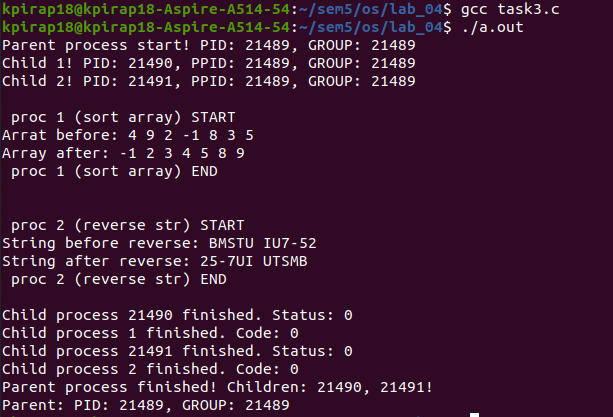
\includegraphics[width=\linewidth]{img/p3.png}
	\caption{Демонстрация работы программы (задание №3).}

	\label{fig:p3}

\end{figure}

\section*{Задание №4}

Предок и потомки обмениваются сообщениями через неименованный
программный канал. Предок ждет завершения своих потомков. Вывод соответствующих сообщений на экран.

\begin{lstlisting}[label=some-code,caption=Использование pipe,language=C]
#include <stdio.h>
#include <unistd.h>
#include <sys/types.h>
#include <sys/wait.h>
#include <string.h>

#define N 2
#define TIME_SLEEP 2
#define LEN 64

#define OK 0
#define ERR_FORK -1
#define ERR_EXEC -1
#define ERR_PIPE -1

#define FORK_FAILURE 1
#define EXEC_FAILURE 2
#define PIPE_FAILURE 3

int main()
{
	int child[N];
	int fd[N];
	char text[LEN] = { 0 };
	char *mes[N] = {"BMSTU IU7-52 Kozlova\n", "ABCDEFG\n"};
	
	if (pipe(fd) == ERR_PIPE)
	{
		perror("Can't pipe!");
		return PIPE_FAILURE;
	}
	
	printf("Parent process start! PID: %d, GROUP: %d\n", getpid(), getpgrp());
	
	for (int i = 0; i < N; i++)
	{
		int child_pid = fork();
		
		if(child_pid == ERR_FORK)
		{
			perror("Can\'t fork()\n");
			return ERR_FORK;
		}
		else if (child_pid == 0)
		{
			close(fd[0]);
			write(fd[1], mes[i], strlen(mes[i]));
            printf("Message %d sent to parent! %s", i + 1, mes[i]);
			
			return OK;
		}        
		else
		{
			child[i] = child_pid;
		}
	}
	
	for (int i = 0; i < N; i++)
	{
		int status;
		int statval = 0;
		
		pid_t child_pid = wait(&status);
		
		printf("Child process %d finished. Status: %d\n", child_pid, status);
		
		if (WIFEXITED(statval))
		{
			printf("Child process %d finished. Code: %d\n", i + 1, WEXITSTATUS(statval));
		}
		else if (WIFSIGNALED(statval))
		{
			printf("Child process %d finished from signal with code: %d\n", i + 1, WTERMSIG(statval));
		}
		else if (WIFSTOPPED(statval))
		{
			printf("Child process %d finished stopped. Number signal: %d\n", i + 1, WSTOPSIG(statval));
		}
	}
	
	printf("\nMessage receive :\n");
	close(fd[1]);
	read(fd[0], text, LEN);
	printf("%s\n", text);
	
	printf("Parent process finished! Children: %d, %d! \nParent: PID: %d, GROUP: %d\n", child[0], child[1], getpid(), getpgrp());
	
	return OK;
}
\end{lstlisting}

\begin{figure}[H]

	\centering

	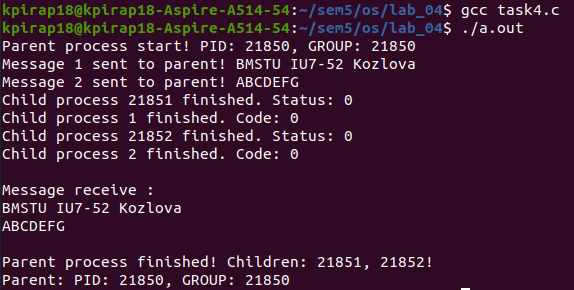
\includegraphics[width=\linewidth]{img/p4.png}
	\caption{Демонстрация работы программы (задание №4).}

	\label{fig:p4}

\end{figure}

\section*{Задание №5}

Предок и потомки обмениваются сообщениями через неименованный программный канал. С помощью сигнала меняется ход выполнения программы. Предок ждет завершения своих потомков. Вывод соответствующих сообщений на экран.

\begin{lstlisting}[label=some-code,caption=Использование ]
#include <stdio.h>
#include <unistd.h>
#include <sys/types.h>
#include <sys/wait.h>
#include <string.h>
#include <stdbool.h> 
#include <signal.h>

#define N 2
#define TIME_SLEEP 2
#define LEN 64

#define OK 0
#define ERR_FORK -1
#define ERR_EXEC -1
#define ERR_PIPE -1

#define FORK_FAILURE 1
#define EXEC_FAILURE 2
#define PIPE_FAILURE 3

_Bool flag = false;


void catch_sig(int sig_num)
{
	flag = true;
	printf("catch_sig: %d\n", sig_num);
}

int main()
{
	int child[N];
	int fd[N];
	char text[LEN] = { 0 };
	char *mes[N] = {"BMSTU IU7-52 Kozlova\n", "ABCDEFG\n"};
	
	if (pipe(fd) == ERR_PIPE)
	{
		perror("Can't pipe!");
		return PIPE_FAILURE;
	}
	
	printf("Parent process start! PID: %d, GROUP: %d\n", getpid(), getpgrp());
	signal(SIGINT, catch_sig);
	sleep(2);
	
	for (int i = 0; i < N; i++)
	{
		int child_pid = fork();
		
		if(child_pid == ERR_FORK)
		{
			perror("Can\'t fork()\n");
			return ERR_FORK;
		}
		else if (child_pid == 0)
		{
			if (flag)
			{
				close(fd[0]);
				write(fd[1], mes[i], strlen(mes[i]));
	            printf("Message %d sent to parent! %s", i + 1, mes[i]);
	
			}
			
			return OK;
		}        
		else
		{
			child[i] = child_pid;
		}
	}
	
	for (int i = 0; i < N; i++)
	{
		int status;
		int statval = 0;
		
		pid_t child_pid = wait(&status);
		
		printf("Child process %d finished. Status: %d\n", child_pid, status);
		
		if (WIFEXITED(statval))
		{
			printf("Child process %d finished. Code: %d\n", i + 1, WEXITSTATUS(statval));
		}
		else if (WIFSIGNALED(statval))
		{
			printf("Child process %d finished from signal with code: %d\n", i + 1, WTERMSIG(statval));
		}
		else if (WIFSTOPPED(statval))
		{
			printf("Child process %d finished stopped. Number signal: %d\n", i + 1, WSTOPSIG(statval));
		}
	}
		
	printf("\nMessage receive :\n");
	close(fd[1]);
	read(fd[0], text, LEN);
	printf("%s\n", text);
	
	printf("Parent process finished! Children: %d, %d! \nParent: PID: %d, GROUP: %d\n", child[0], child[1], getpid(), getpgrp());
	
	return OK;
}
\end{lstlisting}


\begin{figure}[H]

	\centering

	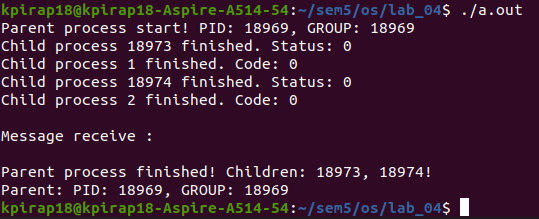
\includegraphics[width=\linewidth]{img/p5.png}
	\caption{Демонстрация работы программы, сигнал не вызывается (задание №5).}

	\label{fig:p5}

\end{figure}


\begin{figure}[H]
	
	\centering
	
	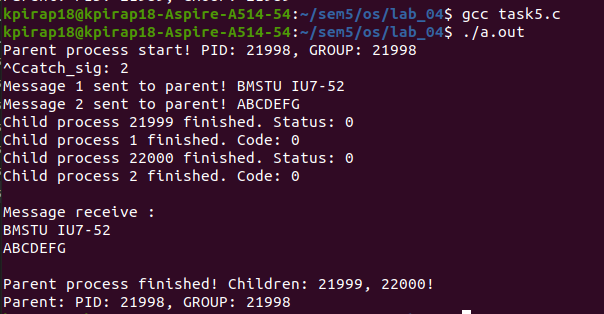
\includegraphics[width=\linewidth]{img/p5_2.png}
	\caption{Демонстрация работы программы, сигнал вызывается (задание №5).}
	
	\label{fig:p5_2}
	
\end{figure}

\bibliographystyle{utf8gost705u}  % стилевой файл для оформления по ГОСТу

\bibliography{51-biblio}          % имя библиографической базы (bib-файла)


\end{document}